\documentclass[1p]{elsarticle_modified}
%\bibliographystyle{elsarticle-num}

%\usepackage[colorlinks]{hyperref}
%\usepackage{abbrmath_seonhwa} %\Abb, \Ascr, \Acal ,\Abf, \Afrak
\usepackage{amsfonts}
\usepackage{amssymb}
\usepackage{amsmath}
\usepackage{amsthm}
\usepackage{scalefnt}
\usepackage{amsbsy}
\usepackage{kotex}
\usepackage{caption}
\usepackage{subfig}
\usepackage{color}
\usepackage{graphicx}
\usepackage{xcolor} %% white, black, red, green, blue, cyan, magenta, yellow
\usepackage{float}
\usepackage{setspace}
\usepackage{hyperref}

\usepackage{tikz}
\usetikzlibrary{arrows}

\usepackage{multirow}
\usepackage{array} % fixed length table
\usepackage{hhline}

%%%%%%%%%%%%%%%%%%%%%
\makeatletter
\renewcommand*\env@matrix[1][\arraystretch]{%
	\edef\arraystretch{#1}%
	\hskip -\arraycolsep
	\let\@ifnextchar\new@ifnextchar
	\array{*\c@MaxMatrixCols c}}
\makeatother %https://tex.stackexchange.com/questions/14071/how-can-i-increase-the-line-spacing-in-a-matrix
%%%%%%%%%%%%%%%

\usepackage[normalem]{ulem}

\newcommand{\msout}[1]{\ifmmode\text{\sout{\ensuremath{#1}}}\else\sout{#1}\fi}
%SOURCE: \msout is \stkout macro in https://tex.stackexchange.com/questions/20609/strikeout-in-math-mode

\newcommand{\cancel}[1]{
	\ifmmode
	{\color{red}\msout{#1}}
	\else
	{\color{red}\sout{#1}}
	\fi
}

\newcommand{\add}[1]{
	{\color{blue}\uwave{#1}}
}

\newcommand{\replace}[2]{
	\ifmmode
	{\color{red}\msout{#1}}{\color{blue}\uwave{#2}}
	\else
	{\color{red}\sout{#1}}{\color{blue}\uwave{#2}}
	\fi
}

\newcommand{\Sol}{\mathcal{S}} %segment
\newcommand{\D}{D} %diagram
\newcommand{\A}{\mathcal{A}} %arc


%%%%%%%%%%%%%%%%%%%%%%%%%%%%%5 test

\def\sl{\operatorname{\textup{SL}}(2,\Cbb)}
\def\psl{\operatorname{\textup{PSL}}(2,\Cbb)}
\def\quan{\mkern 1mu \triangleright \mkern 1mu}

\theoremstyle{definition}
\newtheorem{thm}{Theorem}[section]
\newtheorem{prop}[thm]{Proposition}
\newtheorem{lem}[thm]{Lemma}
\newtheorem{ques}[thm]{Question}
\newtheorem{cor}[thm]{Corollary}
\newtheorem{defn}[thm]{Definition}
\newtheorem{exam}[thm]{Example}
\newtheorem{rmk}[thm]{Remark}
\newtheorem{alg}[thm]{Algorithm}

\newcommand{\I}{\sqrt{-1}}
\begin{document}

%\begin{frontmatter}
%
%\title{Boundary parabolic representations of knots up to 8 crossings}
%
%%% Group authors per affiliation:
%\author{Yunhi Cho} 
%\address{Department of Mathematics, University of Seoul, Seoul, Korea}
%\ead{yhcho@uos.ac.kr}
%
%
%\author{Seonhwa Kim} %\fnref{s_kim}}
%\address{Center for Geometry and Physics, Institute for Basic Science, Pohang, 37673, Korea}
%\ead{ryeona17@ibs.re.kr}
%
%\author{Hyuk Kim}
%\address{Department of Mathematical Sciences, Seoul National University, Seoul 08826, Korea}
%\ead{hyukkim@snu.ac.kr}
%
%\author{Seokbeom Yoon}
%\address{Department of Mathematical Sciences, Seoul National University, Seoul, 08826,  Korea}
%\ead{sbyoon15@snu.ac.kr}
%
%\begin{abstract}
%We find all boundary parabolic representation of knots up to 8 crossings.
%
%\end{abstract}
%\begin{keyword}
%    \MSC[2010] 57M25 
%\end{keyword}
%
%\end{frontmatter}

%\linenumbers
%\tableofcontents
%
\newcommand\colored[1]{\textcolor{white}{\rule[-0.35ex]{0.8em}{1.4ex}}\kern-0.8em\color{red} #1}%
%\newcommand\colored[1]{\textcolor{white}{ #1}\kern-2.17ex	\textcolor{white}{ #1}\kern-1.81ex	\textcolor{white}{ #1}\kern-2.15ex\color{red}#1	}

{\Large $\underline{12n_{0238}~(K12n_{0238})}$}

\setlength{\tabcolsep}{10pt}
\renewcommand{\arraystretch}{1.6}
\vspace{1cm}\begin{tabular}{m{100pt}>{\centering\arraybackslash}m{274pt}}
\multirow{5}{120pt}{
	\centering
	\includegraphics[width=112pt]{../../../GIT/diagram.site/Diagrams/png/2327_12n_0238.png}\\
\ \ \ A knot diagram\footnotemark}&
\allowdisplaybreaks
\textbf{Linearized knot diagam} \\
\cline{2-2}
 &
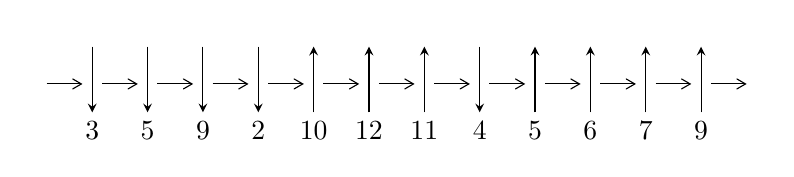
\begin{tikzpicture}[x=20pt, y=17pt]
	% nodes
	\node (C0) at (0, 0) {};
	\node (C1) at (1, 0) {};
	\node (C1U) at (1, +1) {};
	\node (C1D) at (1, -1) {3};

	\node (C2) at (2, 0) {};
	\node (C2U) at (2, +1) {};
	\node (C2D) at (2, -1) {5};

	\node (C3) at (3, 0) {};
	\node (C3U) at (3, +1) {};
	\node (C3D) at (3, -1) {9};

	\node (C4) at (4, 0) {};
	\node (C4U) at (4, +1) {};
	\node (C4D) at (4, -1) {2};

	\node (C5) at (5, 0) {};
	\node (C5U) at (5, +1) {};
	\node (C5D) at (5, -1) {10};

	\node (C6) at (6, 0) {};
	\node (C6U) at (6, +1) {};
	\node (C6D) at (6, -1) {12};

	\node (C7) at (7, 0) {};
	\node (C7U) at (7, +1) {};
	\node (C7D) at (7, -1) {11};

	\node (C8) at (8, 0) {};
	\node (C8U) at (8, +1) {};
	\node (C8D) at (8, -1) {4};

	\node (C9) at (9, 0) {};
	\node (C9U) at (9, +1) {};
	\node (C9D) at (9, -1) {5};

	\node (C10) at (10, 0) {};
	\node (C10U) at (10, +1) {};
	\node (C10D) at (10, -1) {6};

	\node (C11) at (11, 0) {};
	\node (C11U) at (11, +1) {};
	\node (C11D) at (11, -1) {7};

	\node (C12) at (12, 0) {};
	\node (C12U) at (12, +1) {};
	\node (C12D) at (12, -1) {9};
	\node (C13) at (13, 0) {};

	% arrows
	\draw[->,>={angle 60}]
	(C0) edge (C1) (C1) edge (C2) (C2) edge (C3) (C3) edge (C4) (C4) edge (C5) (C5) edge (C6) (C6) edge (C7) (C7) edge (C8) (C8) edge (C9) (C9) edge (C10) (C10) edge (C11) (C11) edge (C12) (C12) edge (C13) ;	\draw[->,>=stealth]
	(C1U) edge (C1D) (C2U) edge (C2D) (C3U) edge (C3D) (C4U) edge (C4D) (C5D) edge (C5U) (C6D) edge (C6U) (C7D) edge (C7U) (C8U) edge (C8D) (C9D) edge (C9U) (C10D) edge (C10U) (C11D) edge (C11U) (C12D) edge (C12U) ;
	\end{tikzpicture} \\
\hhline{~~} \\& 
\textbf{Solving Sequence} \\ \cline{2-2} 
 &
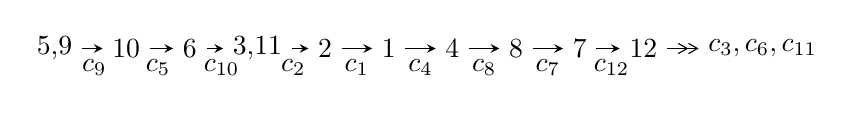
\begin{tikzpicture}[x=23pt, y=7pt]
	% node
	\node (A0) at (-1/8, 0) {5,9};
	\node (A1) at (1, 0) {10};
	\node (A2) at (2, 0) {6};
	\node (A3) at (49/16, 0) {3,11};
	\node (A4) at (33/8, 0) {2};
	\node (A5) at (41/8, 0) {1};
	\node (A6) at (49/8, 0) {4};
	\node (A7) at (57/8, 0) {8};
	\node (A8) at (65/8, 0) {7};
	\node (A9) at (73/8, 0) {12};
	\node (C1) at (1/2, -1) {$c_{9}$};
	\node (C2) at (3/2, -1) {$c_{5}$};
	\node (C3) at (5/2, -1) {$c_{10}$};
	\node (C4) at (29/8, -1) {$c_{2}$};
	\node (C5) at (37/8, -1) {$c_{1}$};
	\node (C6) at (45/8, -1) {$c_{4}$};
	\node (C7) at (53/8, -1) {$c_{8}$};
	\node (C8) at (61/8, -1) {$c_{7}$};
	\node (C9) at (69/8, -1) {$c_{12}$};
	\node (A10) at (11, 0) {$c_{3},c_{6},c_{11}$};

	% edge
	\draw[->,>=stealth]	
	(A0) edge (A1) (A1) edge (A2) (A2) edge (A3) (A3) edge (A4) (A4) edge (A5) (A5) edge (A6) (A6) edge (A7) (A7) edge (A8) (A8) edge (A9) ;
	\draw[->>,>={angle 60}]	
	(A9) edge (A10);
\end{tikzpicture} \\ 

\end{tabular} \\

\footnotetext{
The image of knot diagram is generated by the software ``\textbf{Draw programme}" developed by Andrew Bartholomew(\url{http://www.layer8.co.uk/maths/draw/index.htm\#Running-draw}), where we modified some parts for our purpose(\url{https://github.com/CATsTAILs/LinksPainter}).
}\phantom \\ \newline 
\centering \textbf{Ideals for irreducible components\footnotemark of $X_{\text{par}}$} 
 
\begin{align*}
I^u_{1}&=\langle 
-404722938 u^{20}-1078466313 u^{19}+\cdots+5499202867 b-58406387,\\
\phantom{I^u_{1}}&\phantom{= \langle  }4406297082 u^{20}+8871000551 u^{19}+\cdots+5499202867 a+15450577476,\;u^{21}+2 u^{20}+\cdots+3 u+1\rangle \\
I^u_{2}&=\langle 
b,\;- u^5+u^4+3 u^3-2 u^2+a-2 u-1,\;u^6- u^5-3 u^4+2 u^3+2 u^2+u-1\rangle \\
\\
\end{align*}
\raggedright * 2 irreducible components of $\dim_{\mathbb{C}}=0$, with total 27 representations.\\
\footnotetext{All coefficients of polynomials are rational numbers. But the coefficients are sometimes approximated in decimal forms when there is not enough margin.}
\newpage
\renewcommand{\arraystretch}{1}
\centering \section*{I. $I^u_{1}= \langle -4.05\times10^{8} u^{20}-1.08\times10^{9} u^{19}+\cdots+5.50\times10^{9} b-5.84\times10^{7},\;4.41\times10^{9} u^{20}+8.87\times10^{9} u^{19}+\cdots+5.50\times10^{9} a+1.55\times10^{10},\;u^{21}+2 u^{20}+\cdots+3 u+1 \rangle$}
\flushleft \textbf{(i) Arc colorings}\\
\begin{tabular}{m{7pt} m{180pt} m{7pt} m{180pt} }
\flushright $a_{5}=$&$\begin{pmatrix}0\\u\end{pmatrix}$ \\
\flushright $a_{9}=$&$\begin{pmatrix}1\\0\end{pmatrix}$ \\
\flushright $a_{10}=$&$\begin{pmatrix}1\\- u^2\end{pmatrix}$ \\
\flushright $a_{6}=$&$\begin{pmatrix}u\\- u^3+u\end{pmatrix}$ \\
\flushright $a_{3}=$&$\begin{pmatrix}-0.801261 u^{20}-1.61314 u^{19}+\cdots+8.20107 u-2.80960\\0.0735967 u^{20}+0.196113 u^{19}+\cdots+1.83312 u+0.0106209\end{pmatrix}$ \\
\flushright $a_{11}=$&$\begin{pmatrix}- u^2+1\\u^4-2 u^2\end{pmatrix}$ \\
\flushright $a_{2}=$&$\begin{pmatrix}-0.801261 u^{20}-1.61314 u^{19}+\cdots+8.20107 u-2.80960\\u\end{pmatrix}$ \\
\flushright $a_{1}=$&$\begin{pmatrix}0.265288 u^{20}+0.496064 u^{19}+\cdots+3.71973 u+0.0807825\\-0.0710076 u^{20}-0.0622947 u^{19}+\cdots-1.04835 u-0.0356490\end{pmatrix}$ \\
\flushright $a_{4}=$&$\begin{pmatrix}-0.874858 u^{20}-1.80926 u^{19}+\cdots+6.36794 u-2.82022\\0.0735967 u^{20}+0.196113 u^{19}+\cdots+1.83312 u+0.0106209\end{pmatrix}$ \\
\flushright $a_{8}=$&$\begin{pmatrix}0.0356490 u^{20}+0.000290302 u^{19}+\cdots-0.113612 u-0.941407\\0.0345127 u^{20}-0.0516588 u^{19}+\cdots+0.715083 u+0.265288\end{pmatrix}$ \\
\flushright $a_{7}=$&$\begin{pmatrix}0.0129414 u^{20}+0.219376 u^{19}+\cdots-0.396043 u-1.03717\\0.329095 u^{20}+0.210059 u^{19}+\cdots+1.76622 u+0.634234\end{pmatrix}$ \\
\flushright $a_{12}=$&$\begin{pmatrix}0.336296 u^{20}+0.558359 u^{19}+\cdots+4.76808 u+0.116432\\-0.0710076 u^{20}-0.0622947 u^{19}+\cdots-1.04835 u-0.0356490\end{pmatrix}$\\&\end{tabular}
\flushleft \textbf{(ii) Obstruction class $= -1$}\\~\\
\flushleft \textbf{(iii) Cusp Shapes $= -\frac{19796050041}{5499202867} u^{20}-\frac{34864711542}{5499202867} u^{19}+\cdots+\frac{105657040340}{5499202867} u-\frac{58195456402}{5499202867}$}\\~\\
\newpage\renewcommand{\arraystretch}{1}
\flushleft \textbf{(iv) u-Polynomials at the component}\newline \\
\begin{tabular}{m{50pt}|m{274pt}}
Crossings & \hspace{64pt}u-Polynomials at each crossing \\
\hline $$\begin{aligned}c_{1}\end{aligned}$$&$\begin{aligned}
&u^{21}- u^{20}+\cdots-10 u+1
\end{aligned}$\\
\hline $$\begin{aligned}c_{2},c_{4}\end{aligned}$$&$\begin{aligned}
&u^{21}-7 u^{20}+\cdots-4 u+1
\end{aligned}$\\
\hline $$\begin{aligned}c_{3},c_{8}\end{aligned}$$&$\begin{aligned}
&u^{21}- u^{20}+\cdots+64 u+64
\end{aligned}$\\
\hline $$\begin{aligned}c_{5},c_{9},c_{10}\end{aligned}$$&$\begin{aligned}
&u^{21}+2 u^{20}+\cdots+3 u+1
\end{aligned}$\\
\hline $$\begin{aligned}c_{6},c_{7},c_{11}\end{aligned}$$&$\begin{aligned}
&u^{21}-2 u^{20}+\cdots+u+1
\end{aligned}$\\
\hline $$\begin{aligned}c_{12}\end{aligned}$$&$\begin{aligned}
&u^{21}-8 u^{20}+\cdots+15665 u-2537
\end{aligned}$\\
\hline
\end{tabular}\\~\\
\newpage\renewcommand{\arraystretch}{1}
\flushleft \textbf{(v) Riley Polynomials at the component}\newline \\
\begin{tabular}{m{50pt}|m{274pt}}
Crossings & \hspace{64pt}Riley Polynomials at each crossing \\
\hline $$\begin{aligned}c_{1}\end{aligned}$$&$\begin{aligned}
&y^{21}+53 y^{20}+\cdots+14 y-1
\end{aligned}$\\
\hline $$\begin{aligned}c_{2},c_{4}\end{aligned}$$&$\begin{aligned}
&y^{21}+y^{20}+\cdots-10 y-1
\end{aligned}$\\
\hline $$\begin{aligned}c_{3},c_{8}\end{aligned}$$&$\begin{aligned}
&y^{21}+39 y^{20}+\cdots+71680 y^2-4096
\end{aligned}$\\
\hline $$\begin{aligned}c_{5},c_{9},c_{10}\end{aligned}$$&$\begin{aligned}
&y^{21}-32 y^{20}+\cdots+29 y-1
\end{aligned}$\\
\hline $$\begin{aligned}c_{6},c_{7},c_{11}\end{aligned}$$&$\begin{aligned}
&y^{21}+16 y^{20}+\cdots+29 y-1
\end{aligned}$\\
\hline $$\begin{aligned}c_{12}\end{aligned}$$&$\begin{aligned}
&y^{21}-116 y^{20}+\cdots+451761953 y-6436369
\end{aligned}$\\
\hline
\end{tabular}\\~\\
\newpage\flushleft \textbf{(vi) Complex Volumes and Cusp Shapes}
$$\begin{array}{c|c|c}  
\text{Solutions to }I^u_{1}& \I (\text{vol} + \sqrt{-1}CS) & \text{Cusp shape}\\
 \hline 
\begin{aligned}
u &= -0.533638 + 0.732854 I \\
a &= -0.021350 + 0.475268 I \\
b &= -0.156517 + 0.629640 I\end{aligned}
 & -3.26941 - 2.37868 I & \phantom{-}2.23871 + 4.16638 I \\ \hline\begin{aligned}
u &= -0.533638 - 0.732854 I \\
a &= -0.021350 - 0.475268 I \\
b &= -0.156517 - 0.629640 I\end{aligned}
 & -3.26941 + 2.37868 I & \phantom{-}2.23871 - 4.16638 I \\ \hline\begin{aligned}
u &= \phantom{-}1.270070 + 0.160273 I \\
a &= -0.214865 + 0.848945 I \\
b &= \phantom{-}0.58338 + 1.42040 I\end{aligned}
 & \phantom{-}4.18543 - 2.07978 I & \phantom{-}5.06109 + 1.69933 I \\ \hline\begin{aligned}
u &= \phantom{-}1.270070 - 0.160273 I \\
a &= -0.214865 - 0.848945 I \\
b &= \phantom{-}0.58338 - 1.42040 I\end{aligned}
 & \phantom{-}4.18543 + 2.07978 I & \phantom{-}5.06109 - 1.69933 I \\ \hline\begin{aligned}
u &= \phantom{-}0.578863 + 0.221418 I \\
a &= \phantom{-}0.276951 + 0.590407 I \\
b &= \phantom{-}0.506741 + 0.461302 I\end{aligned}
 & \phantom{-}1.037710 + 0.275110 I & \phantom{-}9.16776 - 1.72750 I \\ \hline\begin{aligned}
u &= \phantom{-}0.578863 - 0.221418 I \\
a &= \phantom{-}0.276951 - 0.590407 I \\
b &= \phantom{-}0.506741 - 0.461302 I\end{aligned}
 & \phantom{-}1.037710 - 0.275110 I & \phantom{-}9.16776 + 1.72750 I \\ \hline\begin{aligned}
u &= -0.602512 + 0.112972 I \\
a &= -0.615716 - 1.104380 I \\
b &= -0.968514 - 0.190025 I\end{aligned}
 & -1.76723 - 2.46823 I & \phantom{-}2.72362 + 4.48751 I \\ \hline\begin{aligned}
u &= -0.602512 - 0.112972 I \\
a &= -0.615716 + 1.104380 I \\
b &= -0.968514 + 0.190025 I\end{aligned}
 & -1.76723 + 2.46823 I & \phantom{-}2.72362 - 4.48751 I \\ \hline\begin{aligned}
u &= -1.378270 + 0.285291 I \\
a &= \phantom{-}0.265526 + 0.752482 I \\
b &= -0.30372 + 1.44468 I\end{aligned}
 & \phantom{-}7.49754 - 2.42009 I & \phantom{-}8.20075 + 2.52746 I \\ \hline\begin{aligned}
u &= -1.378270 - 0.285291 I \\
a &= \phantom{-}0.265526 - 0.752482 I \\
b &= -0.30372 - 1.44468 I\end{aligned}
 & \phantom{-}7.49754 + 2.42009 I & \phantom{-}8.20075 - 2.52746 I\\
 \hline 
 \end{array}$$\newpage$$\begin{array}{c|c|c}  
\text{Solutions to }I^u_{1}& \I (\text{vol} + \sqrt{-1}CS) & \text{Cusp shape}\\
 \hline 
\begin{aligned}
u &= \phantom{-}1.43377 + 0.44455 I \\
a &= -0.268209 + 0.659406 I \\
b &= \phantom{-}0.094833 + 1.327870 I\end{aligned}
 & \phantom{-}3.10341 + 6.65319 I & \phantom{-}3.92005 - 5.62951 I \\ \hline\begin{aligned}
u &= \phantom{-}1.43377 - 0.44455 I \\
a &= -0.268209 - 0.659406 I \\
b &= \phantom{-}0.094833 - 1.327870 I\end{aligned}
 & \phantom{-}3.10341 - 6.65319 I & \phantom{-}3.92005 + 5.62951 I \\ \hline\begin{aligned}
u &= \phantom{-}0.192099 + 0.306787 I \\
a &= \phantom{-}1.15825 - 2.94256 I \\
b &= \phantom{-}0.472659 + 0.611670 I\end{aligned}
 & -4.24122 + 1.01092 I & \phantom{-}0.113832 + 1.103661 I \\ \hline\begin{aligned}
u &= \phantom{-}0.192099 - 0.306787 I \\
a &= \phantom{-}1.15825 + 2.94256 I \\
b &= \phantom{-}0.472659 - 0.611670 I\end{aligned}
 & -4.24122 - 1.01092 I & \phantom{-}0.113832 - 1.103661 I \\ \hline\begin{aligned}
u &= -0.208424\phantom{ +0.000000I} \\
a &= -4.36014\phantom{ +0.000000I} \\
b &= -0.397831\phantom{ +0.000000I}\end{aligned}
 & -1.31628\phantom{ +0.000000I} & -11.0260\phantom{ +0.000000I} \\ \hline\begin{aligned}
u &= -1.83563 + 0.08011 I \\
a &= \phantom{-}0.602185 + 0.714479 I \\
b &= \phantom{-}0.39971 + 2.30587 I\end{aligned}
 & \phantom{-}15.7454 + 0.6574 I & \phantom{-}4.16491 - 0.88898 I \\ \hline\begin{aligned}
u &= -1.83563 - 0.08011 I \\
a &= \phantom{-}0.602185 - 0.714479 I \\
b &= \phantom{-}0.39971 - 2.30587 I\end{aligned}
 & \phantom{-}15.7454 - 0.6574 I & \phantom{-}4.16491 + 0.88898 I \\ \hline\begin{aligned}
u &= \phantom{-}1.86695 + 0.09495 I \\
a &= -0.612105 + 0.689039 I \\
b &= -0.50531 + 2.27337 I\end{aligned}
 & \phantom{-}19.6581 + 4.5242 I & \phantom{-}7.10782 - 2.01921 I \\ \hline\begin{aligned}
u &= \phantom{-}1.86695 - 0.09495 I \\
a &= -0.612105 - 0.689039 I \\
b &= -0.50531 - 2.27337 I\end{aligned}
 & \phantom{-}19.6581 - 4.5242 I & \phantom{-}7.10782 + 2.01921 I \\ \hline\begin{aligned}
u &= -1.88749 + 0.12006 I \\
a &= \phantom{-}0.609399 + 0.663862 I \\
b &= \phantom{-}0.57565 + 2.19938 I\end{aligned}
 & \phantom{-}15.4586 - 9.6359 I & \phantom{-}3.81453 + 4.73258 I\\
 \hline 
 \end{array}$$\newpage$$\begin{array}{c|c|c}  
\text{Solutions to }I^u_{1}& \I (\text{vol} + \sqrt{-1}CS) & \text{Cusp shape}\\
 \hline 
\begin{aligned}
u &= -1.88749 - 0.12006 I \\
a &= \phantom{-}0.609399 - 0.663862 I \\
b &= \phantom{-}0.57565 - 2.19938 I\end{aligned}
 & \phantom{-}15.4586 + 9.6359 I & \phantom{-}3.81453 - 4.73258 I\\
 \hline 
 \end{array}$$\newpage\newpage\renewcommand{\arraystretch}{1}
\centering \section*{II. $I^u_{2}= \langle b,\;- u^5+u^4+3 u^3-2 u^2+a-2 u-1,\;u^6- u^5-3 u^4+2 u^3+2 u^2+u-1 \rangle$}
\flushleft \textbf{(i) Arc colorings}\\
\begin{tabular}{m{7pt} m{180pt} m{7pt} m{180pt} }
\flushright $a_{5}=$&$\begin{pmatrix}0\\u\end{pmatrix}$ \\
\flushright $a_{9}=$&$\begin{pmatrix}1\\0\end{pmatrix}$ \\
\flushright $a_{10}=$&$\begin{pmatrix}1\\- u^2\end{pmatrix}$ \\
\flushright $a_{6}=$&$\begin{pmatrix}u\\- u^3+u\end{pmatrix}$ \\
\flushright $a_{3}=$&$\begin{pmatrix}u^5- u^4-3 u^3+2 u^2+2 u+1\\0\end{pmatrix}$ \\
\flushright $a_{11}=$&$\begin{pmatrix}- u^2+1\\u^4-2 u^2\end{pmatrix}$ \\
\flushright $a_{2}=$&$\begin{pmatrix}u^5- u^4-3 u^3+2 u^2+2 u+1\\- u\end{pmatrix}$ \\
\flushright $a_{1}=$&$\begin{pmatrix}0\\- u\end{pmatrix}$ \\
\flushright $a_{4}=$&$\begin{pmatrix}u^5- u^4-3 u^3+2 u^2+2 u+1\\0\end{pmatrix}$ \\
\flushright $a_{8}=$&$\begin{pmatrix}1\\0\end{pmatrix}$ \\
\flushright $a_{7}=$&$\begin{pmatrix}- u^5+2 u^3+u\\u^5-3 u^3+u\end{pmatrix}$ \\
\flushright $a_{12}=$&$\begin{pmatrix}u\\- u\end{pmatrix}$\\&\end{tabular}
\flushleft \textbf{(ii) Obstruction class $= 1$}\\~\\
\flushleft \textbf{(iii) Cusp Shapes $= u^5-8 u^3+12 u+5$}\\~\\
\newpage\renewcommand{\arraystretch}{1}
\flushleft \textbf{(iv) u-Polynomials at the component}\newline \\
\begin{tabular}{m{50pt}|m{274pt}}
Crossings & \hspace{64pt}u-Polynomials at each crossing \\
\hline $$\begin{aligned}c_{1},c_{2}\end{aligned}$$&$\begin{aligned}
&(u-1)^6
\end{aligned}$\\
\hline $$\begin{aligned}c_{3},c_{8}\end{aligned}$$&$\begin{aligned}
&u^6
\end{aligned}$\\
\hline $$\begin{aligned}c_{4}\end{aligned}$$&$\begin{aligned}
&(u+1)^6
\end{aligned}$\\
\hline $$\begin{aligned}c_{5}\end{aligned}$$&$\begin{aligned}
&u^6+u^5-3 u^4-2 u^3+2 u^2- u-1
\end{aligned}$\\
\hline $$\begin{aligned}c_{6},c_{7}\end{aligned}$$&$\begin{aligned}
&u^6- u^5+3 u^4-2 u^3+2 u^2- u-1
\end{aligned}$\\
\hline $$\begin{aligned}c_{9},c_{10},c_{12}\end{aligned}$$&$\begin{aligned}
&u^6- u^5-3 u^4+2 u^3+2 u^2+u-1
\end{aligned}$\\
\hline $$\begin{aligned}c_{11}\end{aligned}$$&$\begin{aligned}
&u^6+u^5+3 u^4+2 u^3+2 u^2+u-1
\end{aligned}$\\
\hline
\end{tabular}\\~\\
\newpage\renewcommand{\arraystretch}{1}
\flushleft \textbf{(v) Riley Polynomials at the component}\newline \\
\begin{tabular}{m{50pt}|m{274pt}}
Crossings & \hspace{64pt}Riley Polynomials at each crossing \\
\hline $$\begin{aligned}c_{1},c_{2},c_{4}\end{aligned}$$&$\begin{aligned}
&(y-1)^6
\end{aligned}$\\
\hline $$\begin{aligned}c_{3},c_{8}\end{aligned}$$&$\begin{aligned}
&y^6
\end{aligned}$\\
\hline $$\begin{aligned}c_{5},c_{9},c_{10}\\c_{12}\end{aligned}$$&$\begin{aligned}
&y^6-7 y^5+17 y^4-16 y^3+6 y^2-5 y+1
\end{aligned}$\\
\hline $$\begin{aligned}c_{6},c_{7},c_{11}\end{aligned}$$&$\begin{aligned}
&y^6+5 y^5+9 y^4+4 y^3-6 y^2-5 y+1
\end{aligned}$\\
\hline
\end{tabular}\\~\\
\newpage\flushleft \textbf{(vi) Complex Volumes and Cusp Shapes}
$$\begin{array}{c|c|c}  
\text{Solutions to }I^u_{2}& \I (\text{vol} + \sqrt{-1}CS) & \text{Cusp shape}\\
 \hline 
\begin{aligned}
u &= -0.493180 + 0.575288 I \\
a &= -0.858925 - 1.001920 I \\
b &= \phantom{-0.000000 } 0\end{aligned}
 & -4.60518 - 1.97241 I & -3.77811 + 4.83849 I \\ \hline\begin{aligned}
u &= -0.493180 - 0.575288 I \\
a &= -0.858925 + 1.001920 I \\
b &= \phantom{-0.000000 } 0\end{aligned}
 & -4.60518 + 1.97241 I & -3.77811 - 4.83849 I \\ \hline\begin{aligned}
u &= \phantom{-}0.483672\phantom{ +0.000000I} \\
a &= \phantom{-}2.06752\phantom{ +0.000000I} \\
b &= \phantom{-0.000000 } 0\end{aligned}
 & -0.906083\phantom{ +0.000000I} & \phantom{-}9.92530\phantom{ +0.000000I} \\ \hline\begin{aligned}
u &= \phantom{-}1.52087 + 0.16310 I \\
a &= \phantom{-}0.650045 - 0.069710 I \\
b &= \phantom{-0.000000 } 0\end{aligned}
 & \phantom{-}2.05064 + 4.59213 I & \phantom{-}3.28527 - 2.79936 I \\ \hline\begin{aligned}
u &= \phantom{-}1.52087 - 0.16310 I \\
a &= \phantom{-}0.650045 + 0.069710 I \\
b &= \phantom{-0.000000 } 0\end{aligned}
 & \phantom{-}2.05064 - 4.59213 I & \phantom{-}3.28527 + 2.79936 I \\ \hline\begin{aligned}
u &= -1.53904\phantom{ +0.000000I} \\
a &= -0.649754\phantom{ +0.000000I} \\
b &= \phantom{-0.000000 } 0\end{aligned}
 & \phantom{-}6.01515\phantom{ +0.000000I} & \phantom{-}7.06030\phantom{ +0.000000I}\\
 \hline 
 \end{array}$$\newpage
\newpage\renewcommand{\arraystretch}{1}
\centering \section*{ III. u-Polynomials}
\begin{tabular}{m{50pt}|m{274pt}}
Crossings & \hspace{64pt}u-Polynomials at each crossing \\
\hline $$\begin{aligned}c_{1}\end{aligned}$$&$\begin{aligned}
&((u-1)^6)(u^{21}- u^{20}+\cdots-10 u+1)
\end{aligned}$\\
\hline $$\begin{aligned}c_{2}\end{aligned}$$&$\begin{aligned}
&((u-1)^6)(u^{21}-7 u^{20}+\cdots-4 u+1)
\end{aligned}$\\
\hline $$\begin{aligned}c_{3},c_{8}\end{aligned}$$&$\begin{aligned}
&u^6(u^{21}- u^{20}+\cdots+64 u+64)
\end{aligned}$\\
\hline $$\begin{aligned}c_{4}\end{aligned}$$&$\begin{aligned}
&((u+1)^6)(u^{21}-7 u^{20}+\cdots-4 u+1)
\end{aligned}$\\
\hline $$\begin{aligned}c_{5}\end{aligned}$$&$\begin{aligned}
&(u^6+u^5-3 u^4-2 u^3+2 u^2- u-1)(u^{21}+2 u^{20}+\cdots+3 u+1)
\end{aligned}$\\
\hline $$\begin{aligned}c_{6},c_{7}\end{aligned}$$&$\begin{aligned}
&(u^6- u^5+3 u^4-2 u^3+2 u^2- u-1)(u^{21}-2 u^{20}+\cdots+u+1)
\end{aligned}$\\
\hline $$\begin{aligned}c_{9},c_{10}\end{aligned}$$&$\begin{aligned}
&(u^6- u^5-3 u^4+2 u^3+2 u^2+u-1)(u^{21}+2 u^{20}+\cdots+3 u+1)
\end{aligned}$\\
\hline $$\begin{aligned}c_{11}\end{aligned}$$&$\begin{aligned}
&(u^6+u^5+3 u^4+2 u^3+2 u^2+u-1)(u^{21}-2 u^{20}+\cdots+u+1)
\end{aligned}$\\
\hline $$\begin{aligned}c_{12}\end{aligned}$$&$\begin{aligned}
&(u^6- u^5-3 u^4+2 u^3+2 u^2+u-1)(u^{21}-8 u^{20}+\cdots+15665 u-2537)
\end{aligned}$\\
\hline
\end{tabular}\newpage\renewcommand{\arraystretch}{1}
\centering \section*{ IV. Riley Polynomials}
\begin{tabular}{m{50pt}|m{274pt}}
Crossings & \hspace{64pt}Riley Polynomials at each crossing \\
\hline $$\begin{aligned}c_{1}\end{aligned}$$&$\begin{aligned}
&((y-1)^6)(y^{21}+53 y^{20}+\cdots+14 y-1)
\end{aligned}$\\
\hline $$\begin{aligned}c_{2},c_{4}\end{aligned}$$&$\begin{aligned}
&((y-1)^6)(y^{21}+y^{20}+\cdots-10 y-1)
\end{aligned}$\\
\hline $$\begin{aligned}c_{3},c_{8}\end{aligned}$$&$\begin{aligned}
&y^6(y^{21}+39 y^{20}+\cdots+71680 y^2-4096)
\end{aligned}$\\
\hline $$\begin{aligned}c_{5},c_{9},c_{10}\end{aligned}$$&$\begin{aligned}
&(y^6-7 y^5+\cdots-5 y+1)(y^{21}-32 y^{20}+\cdots+29 y-1)
\end{aligned}$\\
\hline $$\begin{aligned}c_{6},c_{7},c_{11}\end{aligned}$$&$\begin{aligned}
&(y^6+5 y^5+\cdots-5 y+1)(y^{21}+16 y^{20}+\cdots+29 y-1)
\end{aligned}$\\
\hline $$\begin{aligned}c_{12}\end{aligned}$$&$\begin{aligned}
&(y^6-7 y^5+17 y^4-16 y^3+6 y^2-5 y+1)\\
&\cdot(y^{21}-116 y^{20}+\cdots+451761953 y-6436369)
\end{aligned}$\\
\hline
\end{tabular}
\vskip 2pc
\end{document}